\section{Computational Approach}
To solve \cref{eq:rotating liouville,eq:radiated envelope} for each of $N_s$ \qds{} at $N_t$ equally-spaced timesteps, we begin with a suitable representation of $\tilde{\vb{P}}(\vb{r}, t)$ in spatial and temporal basis functions, i.e.~
\begin{equation}
  \tilde{\vb{P}}(\vb{r}, t) \equiv \sum_{\ell=0}^{N_s - 1} \sum_{m = 0}^{N_t - 1} \alpha_{\ell m} \vb{S}_\ell(\vb{r}) T_m(t).
  \label{eq:basis functions}
\end{equation}

As the wavelength of any radiation in the system far exceeds the dimensions of any \qd{}, we take $\vb{S}_\ell(\vb{r}) \equiv \vb{d}_\ell \delta(\vb{r} - \vb{r}_\ell)$.
Additionally, such a discretization has the benefit of discretizing \cref{eq:rotating liouville}, forming a set of $N_s$ first-order differential equations coupled through radiative processes.
The $T_m(t)$ require a little more care, however, as they facillitate the derivatives in \cref{eq:radiated envelope} as well as interpolation of $\tilde{\vb{P}}$ for noninteger retardation factors.
We thus make use of a Lagrange interpolation scheme of sufficiently high order as to capture $\tilde{\vb{P}}$, $\partial_t \tilde{\vb{P}}$, and $\partial^2_t \tilde{\vb{P}}$.


\noindent\rule[0.5ex]{\linewidth}{1pt}

Solving \cref{eq:liouville} for each of $n_s$ \qds{} amounts to solving $n_s$ implicitly coupled first-order differential equations in time.
Due to its extreme accuracy and inherent bandlimitedness, we instead make use of the highly-tuned predictor/corrector scheme detailed in~\cite{Glaser2009} to numerically solve \cref{eq:liouville} for each \qd{} in the system.
Approximating $\hat{\rho}_i(t)$ as a weighted sum of complex exponentials, the predictor/corrector scheme proceeds with an extrapolation predictor step,
\begin{equation}
  \hat{\rho}_i(t_{k + 1}) \coloneqq \sum_{\ell = 1}^k \mathcal{P}_\ell^{\qty(0)} \hat{\rho}_i(t_\ell) + \mathcal{P}_\ell^{\qty(1)} \dot{\hat{\rho}}_i(t_\ell),
  \label{eq:predictor}
\end{equation}
and several iterated corrector steps,
\begin{equation}
  \hat{\rho}_i(t_{k + 1}) \coloneqq \mathcal{C}_{k+1}^{\qty(1)} \dot{\hat{\rho}}_i(t_{k + 1}) + \sum_{\ell = 1}^k \mathcal{C}_\ell^{\qty(0)} \hat{\rho}_i(t_i) + \mathcal{C}_\ell^{\qty(1)} \dot{\hat{\rho}}_i(t_\ell).
  \label{eq:corrector}
\end{equation}
where the $\mathcal{P}_\ell^{\qty(0, 1)}$ and $\mathcal{C}_\ell^{\qty(0, 1)}$ coefficients arise from a least-squares solution to a system of complex-valued exponentials on a semidisk in the left complex plane.

The approximation used in \cref{eq:rotating liouville} facilitates large timesteps that encompass many \qds{}.
These dots interact continuously over each timestep, thus a suitable integrator should accommodate multiple scattering events occurring within the same time interval---a feat accomplished naturally through iterated applications of \cref{eq:corrector}.
Moreover, the coupling term in \cref{eq:hamiltonian} and the retardation factor in \cref{eq:total field} add significant complexities, making ``straightforward'' solution methods (such as RK4 or other midstep methods) ill-suited for the problem at hand.
The necessity of a midstep RHS evaluation in RK4 schemes, for instance, proves troublesome; as the RHS to evaluate a given $\dot{\hat{\rho}}_i$ between timesteps depends on every other $\hat{\rho}_j$ at the same timepoint, the system requires either an infinite number of step subdivisions or some sort of extrapolation scheme to advance by $\Delta t$.
As the predictor/corrector method presented here possesses superior accuracy properties alongside a rigorous extrapolation scheme (by construction), it very naturally solves the system described by \cref{eq:rotating liouville,eq:radiated envelope}.

%\subsection{Evaluation of radiated fields}
\begin{figure}
  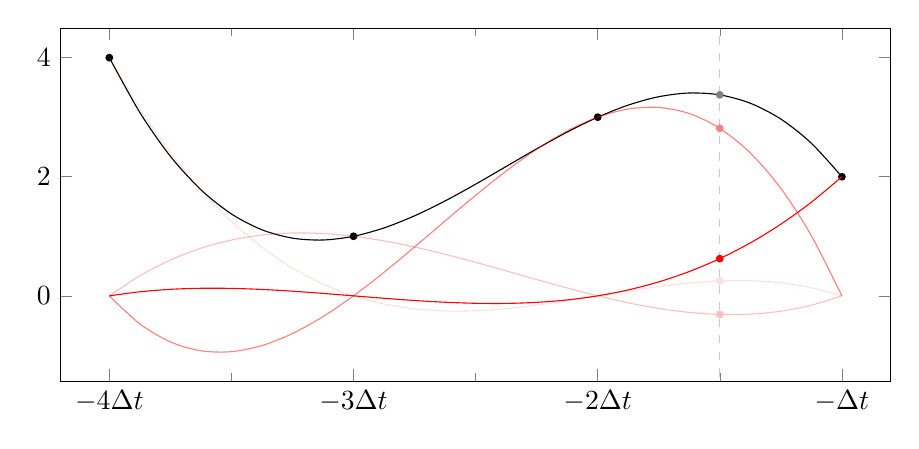
\begin{tikzpicture}
  \begin{axis}[xmin=-4.2, xmax=-0.8, width=\columnwidth, height=0.5\columnwidth,
      xtick={-4, -3, -2, -1},
      minor x tick num={1},
      xticklabels={$-4\Delta t$, $-3\Delta t$, $-2\Delta t$, $-\Delta t$}
  ]

  \addplot[smooth,domain=-4:-1]{2/3*(-3-x)*(-2-x)*(-1-x) + 1/2*(-2-x)*(-1-x)*(4+x) + 3/2*(-1-x)*(3+x)*(4+x) + 1/3*(2+x)*(3+x)*(4+x)};
  \node [fill, black, circle, inner sep=1.0pt] (x1) at (axis cs:-1,2) {};
  \node [fill, black, circle, inner sep=1.0pt] (x2) at (axis cs:-2,3) {};
  \node [fill, black, circle, inner sep=1.0pt] (x2) at (axis cs:-3,1) {};
  \node [fill, black, circle, inner sep=1.0pt] (x2) at (axis cs:-4,4) {};

% Unweighted basis polynomials
  %\draw[dashed, opacity=0.2] (axis cs:-1.2,-10) -- (axis cs:-1.2,10) {};
  %\node [fill, gray, opacity=1.00, circle, inner sep=1.0pt] (pol) at (axis cs:-1.2,2.824) {};

  %\addplot[red, opacity=1.00, smooth, domain=-4:-1]{1/6*(2+x)*(3+x)*(4+x)};
  %\addplot[red, opacity=0.50, smooth, domain=-4:-1]{1/2*(-1-x)*(3+x)*(4+x)};
  %\addplot[red, opacity=0.25, smooth, domain=-4:-1]{1/2*(-2-x)*(-1-x)*(4+x)};
  %\addplot[red, opacity=0.12, smooth, domain=-4:-1]{1/6*(-3-x)*(-2-x)*(-1-x)};

  %\node[fill, red,            circle, inner sep=1.0pt] (p1) at (axis cs:-1.2,0.672) {};
  %\node[fill, red!50!white,   circle, inner sep=1.0pt] (p2) at (axis cs:-1.2,0.504) {};
  %\node[fill, red!25!white,   circle, inner sep=1.0pt] (p3) at (axis cs:-1.2,-0.224) {};
  %\node[fill, red!12.5!white, circle, inner sep=1.0pt] (p4) at (axis cs:-1.2,0.048) {};

% Weighted basis polynomials
  \draw[dashed, opacity=0.2] (axis cs:-1.5,-10) -- (axis cs:-1.5,10) {};
  \node [fill, gray, opacity=1.00, circle, inner sep=1.0pt] (pol) at (axis cs:-1.5,3.375) {};

  \addplot[red, opacity=1.00, smooth, domain=-4:-1]{1/3*(2+x)*(3+x)*(4+x)};
  \addplot[red, opacity=0.50, smooth, domain=-4:-1]{3/2*(-1-x)*(3+x)*(4+ x)};
  \addplot[red, opacity=0.25, smooth, domain=-4:-1]{1/2*(-2-x)*(-1-x)*(4+x)};
  \addplot[red, opacity=0.12, smooth, domain=-4:-1]{2/3*(-3-x)*(-2-x)*(-1-x)};

  \node[fill, red,            circle, inner sep=1.0pt] (p1) at (axis cs:-1.5,0.625) {};
  \node[fill, red!50!white,   circle, inner sep=1.0pt] (p2) at (axis cs:-1.5,2.8125) {};
  \node[fill, red!25!white,   circle, inner sep=1.0pt] (p3) at (axis cs:-1.5,-0.3125) {};
  \node[fill, red!12.5!white, circle, inner sep=1.0pt] (p4) at (axis cs:-1.5,0.25) {};

  \end{axis}
\end{tikzpicture}

  \caption{\label{fig:interpolation}Illustration of interpolation with four basis polynomials.
    An assumed signal takes $1.5\Delta t$ to travel from between points.
    Evaluations of the basis polynomials (and their derivatives) need only occur once between each pair of points (red dots) due to their translational invariance.
    The interpolated signal then becomes a sum of these values weighted by the known samples (black dots).
  }
\end{figure}

To evaluate \cref{eq:radiated envelope} between every pair of points we make use of variable-order Lagrange interpolation scheme.
Such a scheme easily accommodates both retardation effects between \qds{} separated by a non-integer number of timesteps as well as the first and second time derivatives of $\vb{P}$.
To make the interpolation calculation as efficient as possible at each timestep, we store only an history index (integer) and several interpolation coefficients (complex doubles) for every pair of \qds{}.
The history index corresponds to $\lfloor \abs{\Delta \vb{r}}/(c \, \Delta t) \rfloor$ and gives the start of the ``interpolation window'' used to reconstruct $\tilde{E}$ (\cref{fig:interpolation}).
The interpolation coefficients hold $\vb{d}_i \cdot \tilde{\vb{E}}_\text{rad} \cdot \vb{d}_j$ for an interpolatory representation of the integrand in \cref{eq:radiated envelope} (i.e.\ $\tilde{\vb{P}}$ becomes the basis polynomials evaluated at the correct time and contains none of the system dynamics).
